\documentclass[]{book}
\usepackage{lmodern}
\usepackage{amssymb,amsmath}
\usepackage{ifxetex,ifluatex}
\usepackage{fixltx2e} % provides \textsubscript
\ifnum 0\ifxetex 1\fi\ifluatex 1\fi=0 % if pdftex
  \usepackage[T1]{fontenc}
  \usepackage[utf8]{inputenc}
\else % if luatex or xelatex
  \ifxetex
    \usepackage{mathspec}
  \else
    \usepackage{fontspec}
  \fi
  \defaultfontfeatures{Ligatures=TeX,Scale=MatchLowercase}
\fi
% use upquote if available, for straight quotes in verbatim environments
\IfFileExists{upquote.sty}{\usepackage{upquote}}{}
% use microtype if available
\IfFileExists{microtype.sty}{%
\usepackage{microtype}
\UseMicrotypeSet[protrusion]{basicmath} % disable protrusion for tt fonts
}{}
\usepackage[margin=1in]{geometry}
\usepackage{hyperref}
\hypersetup{unicode=true,
            pdftitle={Case Studies in Reproducible Research: a spring seminar at UCSC},
            pdfauthor={Eric C. Anderson, Kristen C. Ruegg, Tina Cheng, and the students of EEB 295},
            pdfborder={0 0 0},
            breaklinks=true}
\urlstyle{same}  % don't use monospace font for urls
\usepackage{natbib}
\bibliographystyle{apalike}
\usepackage{color}
\usepackage{fancyvrb}
\newcommand{\VerbBar}{|}
\newcommand{\VERB}{\Verb[commandchars=\\\{\}]}
\DefineVerbatimEnvironment{Highlighting}{Verbatim}{commandchars=\\\{\}}
% Add ',fontsize=\small' for more characters per line
\usepackage{framed}
\definecolor{shadecolor}{RGB}{248,248,248}
\newenvironment{Shaded}{\begin{snugshade}}{\end{snugshade}}
\newcommand{\KeywordTok}[1]{\textcolor[rgb]{0.13,0.29,0.53}{\textbf{{#1}}}}
\newcommand{\DataTypeTok}[1]{\textcolor[rgb]{0.13,0.29,0.53}{{#1}}}
\newcommand{\DecValTok}[1]{\textcolor[rgb]{0.00,0.00,0.81}{{#1}}}
\newcommand{\BaseNTok}[1]{\textcolor[rgb]{0.00,0.00,0.81}{{#1}}}
\newcommand{\FloatTok}[1]{\textcolor[rgb]{0.00,0.00,0.81}{{#1}}}
\newcommand{\ConstantTok}[1]{\textcolor[rgb]{0.00,0.00,0.00}{{#1}}}
\newcommand{\CharTok}[1]{\textcolor[rgb]{0.31,0.60,0.02}{{#1}}}
\newcommand{\SpecialCharTok}[1]{\textcolor[rgb]{0.00,0.00,0.00}{{#1}}}
\newcommand{\StringTok}[1]{\textcolor[rgb]{0.31,0.60,0.02}{{#1}}}
\newcommand{\VerbatimStringTok}[1]{\textcolor[rgb]{0.31,0.60,0.02}{{#1}}}
\newcommand{\SpecialStringTok}[1]{\textcolor[rgb]{0.31,0.60,0.02}{{#1}}}
\newcommand{\ImportTok}[1]{{#1}}
\newcommand{\CommentTok}[1]{\textcolor[rgb]{0.56,0.35,0.01}{\textit{{#1}}}}
\newcommand{\DocumentationTok}[1]{\textcolor[rgb]{0.56,0.35,0.01}{\textbf{\textit{{#1}}}}}
\newcommand{\AnnotationTok}[1]{\textcolor[rgb]{0.56,0.35,0.01}{\textbf{\textit{{#1}}}}}
\newcommand{\CommentVarTok}[1]{\textcolor[rgb]{0.56,0.35,0.01}{\textbf{\textit{{#1}}}}}
\newcommand{\OtherTok}[1]{\textcolor[rgb]{0.56,0.35,0.01}{{#1}}}
\newcommand{\FunctionTok}[1]{\textcolor[rgb]{0.00,0.00,0.00}{{#1}}}
\newcommand{\VariableTok}[1]{\textcolor[rgb]{0.00,0.00,0.00}{{#1}}}
\newcommand{\ControlFlowTok}[1]{\textcolor[rgb]{0.13,0.29,0.53}{\textbf{{#1}}}}
\newcommand{\OperatorTok}[1]{\textcolor[rgb]{0.81,0.36,0.00}{\textbf{{#1}}}}
\newcommand{\BuiltInTok}[1]{{#1}}
\newcommand{\ExtensionTok}[1]{{#1}}
\newcommand{\PreprocessorTok}[1]{\textcolor[rgb]{0.56,0.35,0.01}{\textit{{#1}}}}
\newcommand{\AttributeTok}[1]{\textcolor[rgb]{0.77,0.63,0.00}{{#1}}}
\newcommand{\RegionMarkerTok}[1]{{#1}}
\newcommand{\InformationTok}[1]{\textcolor[rgb]{0.56,0.35,0.01}{\textbf{\textit{{#1}}}}}
\newcommand{\WarningTok}[1]{\textcolor[rgb]{0.56,0.35,0.01}{\textbf{\textit{{#1}}}}}
\newcommand{\AlertTok}[1]{\textcolor[rgb]{0.94,0.16,0.16}{{#1}}}
\newcommand{\ErrorTok}[1]{\textcolor[rgb]{0.64,0.00,0.00}{\textbf{{#1}}}}
\newcommand{\NormalTok}[1]{{#1}}
\usepackage{longtable,booktabs}
\usepackage{graphicx,grffile}
\makeatletter
\def\maxwidth{\ifdim\Gin@nat@width>\linewidth\linewidth\else\Gin@nat@width\fi}
\def\maxheight{\ifdim\Gin@nat@height>\textheight\textheight\else\Gin@nat@height\fi}
\makeatother
% Scale images if necessary, so that they will not overflow the page
% margins by default, and it is still possible to overwrite the defaults
% using explicit options in \includegraphics[width, height, ...]{}
\setkeys{Gin}{width=\maxwidth,height=\maxheight,keepaspectratio}
\IfFileExists{parskip.sty}{%
\usepackage{parskip}
}{% else
\setlength{\parindent}{0pt}
\setlength{\parskip}{6pt plus 2pt minus 1pt}
}
\setlength{\emergencystretch}{3em}  % prevent overfull lines
\providecommand{\tightlist}{%
  \setlength{\itemsep}{0pt}\setlength{\parskip}{0pt}}
\setcounter{secnumdepth}{5}
% Redefines (sub)paragraphs to behave more like sections
\ifx\paragraph\undefined\else
\let\oldparagraph\paragraph
\renewcommand{\paragraph}[1]{\oldparagraph{#1}\mbox{}}
\fi
\ifx\subparagraph\undefined\else
\let\oldsubparagraph\subparagraph
\renewcommand{\subparagraph}[1]{\oldsubparagraph{#1}\mbox{}}
\fi

%%% Use protect on footnotes to avoid problems with footnotes in titles
\let\rmarkdownfootnote\footnote%
\def\footnote{\protect\rmarkdownfootnote}

%%% Change title format to be more compact
\usepackage{titling}

% Create subtitle command for use in maketitle
\newcommand{\subtitle}[1]{
  \posttitle{
    \begin{center}\large#1\end{center}
    }
}

\setlength{\droptitle}{-2em}
  \title{Case Studies in Reproducible Research: a spring seminar at UCSC}
  \pretitle{\vspace{\droptitle}\centering\huge}
  \posttitle{\par}
  \author{Eric C. Anderson, Kristen C. Ruegg, Tina Cheng, and the students of EEB
295}
  \preauthor{\centering\large\emph}
  \postauthor{\par}
  \predate{\centering\large\emph}
  \postdate{\par}
  \date{2017-04-07}

\usepackage{booktabs}
\usepackage{amsthm}
\makeatletter
\def\thm@space@setup{%
  \thm@preskip=8pt plus 2pt minus 4pt
  \thm@postskip=\thm@preskip
}
\makeatother

\usepackage{amsthm}
\newtheorem{theorem}{Theorem}[chapter]
\newtheorem{lemma}{Lemma}[chapter]
\theoremstyle{definition}
\newtheorem{definition}{Definition}[chapter]
\newtheorem{corollary}{Corollary}[chapter]
\newtheorem{proposition}{Proposition}[chapter]
\theoremstyle{definition}
\newtheorem{example}{Example}[chapter]
\theoremstyle{remark}
\newtheorem*{remark}{Remark}
\begin{document}
\maketitle

{
\setcounter{tocdepth}{1}
\tableofcontents
}
\chapter{Course Overview}\label{course-overview}

This is the home of the notes for a proposed course in data analysis and
reproducible research using R, Rstudio, and GitHub.

The seminar is called, ``Case Studies in Reproducible Research,'' but we
utter that title with the caveat that, although the organizers have
quite a few case studies they could spin up for this course, the case
studies we will be studying in this course are going to be actual
research projects that \emph{you}---the participants---are working on.
You're gonna bring 'em, and we are going to collectively help you
wrassle them into a reasonable and reproducible data analysis. In the
process we will touch on a number of elements of data analysis with R.

We will be working through a healthy chunk of the material in Garrett
Grolemund and Hadley Wickham's book, \href{http://r4ds.had.co.nz/}{R for
Data Science}, which is readable for free at the link above. We intend
to use a handful of our own data sets each week to illustrate points
from the book and show the material in action on real data sets.

This is not intended as a ``first course in R''. Students coming to the
course should have at least a modicum of familiarity with using R, and
we will launch more directly into using the tools of the
\href{http://tidyverse.org/}{tidyverse}. EEB students with little or no
experience in R might be interested in sitting in with Giacomo
Bernardi's lab group on Mondays at 3PM in the COH library. They are
conducting a Bio 295 seminar, working through ``a super basic book that
takes the very first steps into R.''

For the interested, these materials were all prepared using RStudio's
\href{https://bookdown.org/}{bookdown} package. The RStudio project in
which it lives is hosted on eriq's GitHub page
\href{https://github.com/eriqande/rep-res-eeb-2017}{here}

\section{Meeting Times, Location,
Requirements}\label{meeting-times-location-requirements}

Intended to be Friday afternoons, 1:45--3:15 PM in the
library/conference room at Long Marine Lab.

Students must bring a laptop to do examples during the seminar, and all
students are expected to have a data set that they are in the midst of
analyzing (or upon which they hope to commence analysis soon!) for a
research project. We will

\section{The origin of this seminar}\label{the-origin-of-this-seminar}

The idea for this course was floated by Tina Cheng who was planning to
lead a seminar in spring 2017 based in part on Eric C. Anderson's
\href{http://eriqande.github.io/rep-res-web/}{``Reproducible Research
Course''}, taught at the Southwest Fisheries Science Center in the fall
of 2014. Although going over those notes might have been a reasonable
exercise, it turns out that a lot has changed in the world of data
analysis since fall 2014, and the notes from that course are, today, a
little bit dated.

We have been particularly excited by the ascendancy of Hadley Wickham's
\href{http://tidyverse.org/}{tidyverse} approach to data analysis, and
the tremendous development of a variety of tools developed by
\href{https://www.rstudio.com/}{RStudio} for integrating report
generation and data analysis into reproducible workflows. In fact, Eric
has been saying for the last year that if he were to teach another
course on data analysis it would be structured completely differently
than his \href{http://eriqande.github.io/rep-res-web/}{``Reproducible
Research Course''}. So, it was clearly time for him to stop talking and
help put together an updated and different course.

At the same time, in working on our own projects and in helping others,
we have consistently found that the most effective way for anyone to
learn data analysis is to ensure that it is immediately relevant to
whatever ongoing research project is currently consuming them.
Therefore, in the current seminar, we are hoping to spend at least half
of our time ``workshopping'' the data sets that seminar participants are
actually involved in analyzing. Together we will help students wrestle
their data, analyses, and ideas into a single, well-organized RStudio
project under version control with git. Therefore, every student should
come to this course with a data set and an associated analysis project.

\section{Course Organizers}\label{course-organizers}

\begin{description}
\item[Kristen C. Ruegg]
Kristen is a conservation geneticist who specializes in the application
of genome-wide data to understand population level processes and inform
management, with a particular focus on migratory birds. She has has been
enlightened to the powers of the ``tidyverse'' over the last couple of
years (mostly through the constant insistence of her enthusiastic
husband Eric Anderson) and is looking forward to becoming more fluid in
its application over the course of the quarter. Her main role in this
course will be to help with the course design and logistics and help
reign Eric in when he has started to orbit into some obscure realm of
statistical nuance.
\item[Eric C. Anderson]
Eric trained as a statistician who specializes in genetic data. Since
2003 he has worked at the NMFS Southwest Fisheries Science Center in
Santa Cruz. Although much of his statistical research involves the
development of computationally intensive methods for specialized
analyses of genetic data, he has been involved in a variety of data
analysis projects at NMFS and with collaborators worldwide. Eric was an
early adherent to reproducible research principles and continues, as
such, performing most of his research and data analysis in the open and
publicly available on GitHub (find his GitHub page
\href{https://github.com/eriqande}{here}). In 2014, he taught the
\href{http://eriqande.github.io/rep-res-web/}{``Reproducible Research
Course''} at NMFS, and is excited to provide an updated version,
focusing more, this time, on the recently developed ``tidyverse''.
\item[Tina Cheng]
Tina is a graduate student in EEB. She is going to be leading the
session during the first week of the course when Kristen and Eric are
still on spring break, and then she is going to be joining in on the fun
with us for the remainder of the quarter until she has to travel off to
Baja, TA-ing the ``supercourse'' during the last four weeks of the
quarter.
\end{description}

\section{Course Goals}\label{course-goals}

The goal of this course is for scientists, researchers, and students to
learn to:

\begin{itemize}
\tightlist
\item
  properly store, manage, and distribute their data in a \emph{tidy}
  format
\item
  consolidate their digital research materials and analyses into
  well-organized RStudio projects.
\item
  use the tools of the tidyverse to manipulate and analyze those data
  sets
\item
  integrate data analysis with report generation and article preparation
  using the Rmarkdown format and using
  \href{http://rmarkdown.rstudio.com/r_notebooks.html}{R Notebooks}
\item
  use git version control software and GitHub to effectively manage data
  and source code, collaborate efficiently with other researchers, and
  neatly package their research.
\end{itemize}

By the end of the course, the hope is that we will all have mastered
strategies allowing us to use the above-listed, freely-available and
open-source tools for conducting research in a reproducible fashion. The
ideal we will be striving for is to be able to start from a raw data set
and then write a computer program that conducts all the cleaning,
manipulation, and analysis of the data, and presentation of the results,
in an automated fashion. Carrying out analysis and report-generation in
this way carries a number of advantages to the researcher:

\begin{enumerate}
\def\labelenumi{\arabic{enumi}.}
\tightlist
\item
  Newly-collected data can be integrated easily into your analysis.
\item
  If a mistake is found in one section of your analysis, it is not
  terribly onerous to correct it and then re-run all the downstream
  analyses.
\item
  Revising a manuscript to address referee comments can be done quickly.
\item
  Years after publication, the exact steps taken to analyze the data
  will still be available should anyone ask you how, exactly, you did an
  analysis!
\item
  If you have to conduct similar analyses and produce similar reports on
  a regular bias with new data each time, you might be able to do this
  readily by merely updating your data and then automatically producing
  the entire report.
\item
  If someone finds an error in your work, they can fix it and then
  easily show you exactly what they did to fix it.
\end{enumerate}

Additionally, packaging one's research in a reproducible fashion is
beneficial to the research community. Others that would like to confirm
your results can do so easily. If someone has concerns about exactly how
a particular analysis was carried out, they can find the precise details
in the code that you wrote to do it. Someone wanting to apply your
methods to their own data can easily do so, and, finally, if we are all
transparent and open about the methods that we use, then everyone can
learn more quickly from their colleagues.

In many fields today, publication of research requires the submission of
the original data to a publicly-available data repository. Currently,
several journals require that all analyses be packaged in a clear and
transparent fashion for easy reproduction of the results, and I predict
that trend will continue until most, if not all, journals will require
that data analyses be available in easily reproduced formats. This
course will help scientists prepare themselves for this eventuality. In
the process, you will probably find that conducting your research in a
reproducible fashion helps you work more efficiently (and perhaps even
more enjoyably!)

\section{Weekly Syllabus}\label{weekly-syllabus}

\subsection{Week 1 --- Introduction and Getting Your Workspace Set
Up}\label{week-1-introduction-and-getting-your-workspace-set-up}

\begin{itemize}
\tightlist
\item
  At the end of this session we want to make sure that everyone has R,
  RStudio, and Git installed on their systems, and that they are working
  as expected.
\item
  Additionally, everyoneshould have a free account on GitHub.
\item
  And finally we need everyone's email address.
\end{itemize}

Some things to do:

\begin{itemize}
\tightlist
\item
  Get Rstudio cheat Sheets!
\item
  Assemble data into a project
\item
  Get private GitHub repos
\end{itemize}

Eric! You need to make an example project repo.

\subsection{Week 2 --- RStudio project organization; using git and
GitHub; Quick
RMarkdown}\label{week-2-rstudio-project-organization-using-git-and-github-quick-rmarkdown}

After this, students are going to have to put their own data into their
own repositories and write a README.Rmd and make a README.md out of it.

\subsection{Week 3 --- Tibbles. Reading data in. Data
rectangling}\label{week-3-tibbles.-reading-data-in.-data-rectangling}

\begin{itemize}
\tightlist
\item
  Reading data into the data frames.
\item
  read.table and read.csv
\item
  tibbles
\item
  The readr package
\item
  Data types in the different columns and quick data sanity checks.
\item
  A few different gotcha's
\item
  Saving and reading data in R formats. \texttt{saveRDS} and
  \texttt{readRDS}.
\end{itemize}

\subsection{Week 4 ---}\label{week-4}

\chapter{Week One Meeting}\label{week1}

Tina is going to be helping everyone get their systems all set up. After
that we will have everyone clone an RStudio project from GitHub to see
how easy that is.

\section{Software Installation}\label{software-installation}

\begin{enumerate}
\def\labelenumi{\arabic{enumi}.}
\item
  \textbf{RStudio:} We want the latest ``development'' version of
  RStudio becuase it has features that we may want to use during this
  course. Get it from
  \url{https://www.rstudio.com/products/rstudio/download/preview/} and
  install the appropriate one for your OS.
\item
  \textbf{R:} Let's make sure that we are all using the latest version
  of R. On March 7, 2017, version 3.3.3 was released. Go to
  \url{https://cran.r-project.org/} and find the download link for your
  computer system. Download it and install it.
\item
  \textbf{bookdown:} This package is what I used to create these course
  notes. Getting it automatically installs a lot of other packages that
  are useful for authoring reproducible research. We want the latest
  development version, which can be obtained from GitHub by issuing the
  following commans at the R prompt (i.e.~in the console window of
  RStudio:)

\begin{Shaded}
\begin{Highlighting}[]
\KeywordTok{install.packages}\NormalTok{(}\StringTok{"devtools"}\NormalTok{)  }
\NormalTok{devtools::}\KeywordTok{install_github}\NormalTok{(}\StringTok{"rstudio/bookdown"}\NormalTok{)}
\end{Highlighting}
\end{Shaded}
\item
  Install \textbf{other packages} that we are going to be needing in the
  first few weeks. If you don't know how to install packages, ask Tina
  and she can show you. Install: \texttt{tidyverse}, and
  \texttt{stringr}.
\item
  Make sure that \textbf{git} is up and running on your system.

  \begin{itemize}
  \item
    If you are using a Mac with a reasonably new OS, you should be able
    to just open the Terminal application
    (\texttt{/Applications/Utilities/Terminal}) and type ``git'' at the
    command line. If you have \texttt{git} it will say something that
    starts like:

\begin{Shaded}
\begin{Highlighting}[]
    \KeywordTok{usage}\NormalTok{: git [--version] [--help] [-C }\KeywordTok{<}\NormalTok{path}\KeywordTok{>}\NormalTok{] [-c name=value]}
   \NormalTok{[}\KeywordTok{--exec-path}\NormalTok{[=}\KeywordTok{<}\NormalTok{path}\KeywordTok{>}\NormalTok{]] [--html-path] [--man-path] [--info-path]}
   \NormalTok{[}\KeywordTok{-p} \KeywordTok{|} \KeywordTok{--paginate} \KeywordTok{|} \KeywordTok{--no-pager}\NormalTok{] [--no-replace-objects] [--bare]}
   \NormalTok{[}\KeywordTok{--git-dir}\NormalTok{=}\KeywordTok{<}\NormalTok{path}\KeywordTok{>}\NormalTok{] [--work-tree=}\KeywordTok{<}\NormalTok{path}\KeywordTok{>}\NormalTok{] [--namespace=}\KeywordTok{<}\NormalTok{name}\KeywordTok{>}\NormalTok{]}
   \KeywordTok{<command>} \NormalTok{[}\KeywordTok{<}\NormalTok{args}\KeywordTok{>}\NormalTok{]}

\KeywordTok{These} \NormalTok{are common Git commands used in various situations:}

\KeywordTok{start} \NormalTok{a working area (see also: git help tutorial)}
   \KeywordTok{clone}      \NormalTok{Clone a repository into a new directory}
   \KeywordTok{etc.} \NormalTok{etc. etc.}
\end{Highlighting}
\end{Shaded}

    If you do not have \texttt{git} then it should pop up a little thing
    asking if you would like to install a reduced set of developer
    tools. You do. Click OK. \textbf{NOTE} Instead of a pop up it might
    say something like, ``xcrun Error: invalid active developer path.
    etc. etc\ldots{}''. In that case, you can install a fresh set of
    command line tools by typing this at the command line:

\begin{verbatim}
xcode-select --install
\end{verbatim}
  \item
    If you are using a PC, I can't be as much help, but you can find
    links with instructions on how to download \texttt{git} for a PC
    \href{https://support.rstudio.com/hc/en-us/articles/200532077-Version-Control-with-Git-and-SVN}{here}.
  \item
    If you are using Linux then we will assume you know how to get
    \texttt{git} or that you already have it.
  \end{itemize}
\end{enumerate}

\section{Get an account on GitHub}\label{get-an-account-on-github}

If you don't already have an account on GitHub, go to \url{github.com}
and click the ``sign up'' link near upper right of the page. It is
pretty self-explanatory. Go ahead and get a \textbf{free} account. There
is nothing to pay for here!

\subsection{Private repositories}\label{private-repositories}

\emph{If you are a graduate student} and you do not feel comfortable
posting your data on a public site like GitHub, then you should request
some private repositories from GitHub. GitHub has a great deal for
academic users like students: free private repositories. Please go to
\url{https://education.github.com/pack} to sign up for your free student
pack.

\section{Open an RStudio Project from
GitHub}\label{open-an-rstudio-project-from-github}

I am going to have everyone use RStudio and GitHub to clone and open an
RStudio project that I prepared as a template so that people can see how
I would like them to start putting together their own projects.

To open this project, from RStudio, go to the menu option
``File-\textgreater{}New Project\ldots{}''. Then from the resulting
dialog, choose ``Version Control''. Then choose ``Git''. Then it asks
for a ``repository URL''. Supply this:
\texttt{https://github.com/eriqande/rep-res-coho-example} and leave the
``Project Directory Name'' empty. And then choose a directory in which
to put it and click OK.

Bam! That will pull the RStudio project off of GitHub, make a local
clone of it on your hard drive and open.

Once you have done that. Open \texttt{README.Rmd} within the project,
and click the ``knit'' button which should be present near the top left
of the editor window.

That is how you convert an R Markdown README to README.md which is easy
to read and see on GitHub.

If you want to see what the project repository looks like on GitHub,
have a look at \url{https://github.com/eriqande/rep-res-coho-example}.

\section{Assignment for next week: Create an RStudio Project with Your
Own
Data}\label{assignment-for-next-week-create-an-rstudio-project-with-your-own-data}

Your mission for the following week---i.e., please have this done (or as
done as you can get it) by Friday, April 14, 2017---is to prepare an
RStudio project with your own data set, and provide some background
about the data and the ways that you would like to analyze it. The
``rep-res-coho-example'' is an example of what I have in mind for this.
You should use the README.Rmd from that project as a template for your
own README.Rmd. (To do this you can just copy the README.Rmd file into
the top level of your project directory and then edit it to reflect your
own data and project.)

To do all this you are going to want to make your own project. Do that
like this:

\begin{enumerate}
\def\labelenumi{\arabic{enumi}.}
\tightlist
\item
  In RStudio, choose ``File-\textgreater{}New Project\ldots{}''
\item
  Then choose ``New Directory'' and then choose ``Empty Project''
\item
  In the next dialog, choose a name (\emph{it is best to use only
  letters, numbers, dashes, and underscores, and include no spaces in
  the name}) for it \textbf{and be sure to click the ``Create a git
  repository'' button}.\\
\item
  Then click ``Create Project''.
\end{enumerate}

That should give you a new project. Here are some guidelines for putting
your own data in there

\begin{itemize}
\tightlist
\item
  Put all of your data in a directory named \texttt{data} in your
  project.
\item
  CSV (comma separated values) is probably the best format to use. It is
  text-readable without proprietary software (unlike an Excel file);
  however if you need to look at it in a tabular way with Excel, (gasp),
  you can do that easily. Tab-delimited text works if you have that, but
  CSV is preferred.
\item
  Use only letters, numbers, dashes, and underscores for the file names,
  (and periods for their extensions, i.e., \texttt{.csv})
\item
  Give a brief description of your data in the README.Rmd.
\end{itemize}

\section{Reading for next week}\label{reading-for-next-week}

This week (before Friday, April 14, 2017), please read the following
sections of the R for Data Science book

\begin{itemize}
\tightlist
\item
  \href{http://r4ds.had.co.nz/workflow-basics.html}{Workflow basics}:
  super basic review on how R works.
\item
  \href{http://r4ds.had.co.nz/workflow-projects.html}{Workflow:
  projects}: info about organizing RStudio projects.
\item
  \href{http://r4ds.had.co.nz/workflow-scripts.html}{Workflow: scripts}:
  how to evaluate code in scripts.
\item
  \href{http://r4ds.had.co.nz/tibbles.html}{tibbles}: a streamlined data
  frame format.
\item
  \href{http://r4ds.had.co.nz/data-import.html}{data import} This is our
  key reading for the week.
\end{itemize}

When you are done with the \emph{Data Import} reading, take a whack at
writing some code to read the data files in your project into a variable
(or several variables).

\chapter{Applications}\label{applications}

Some \emph{significant} applications are demonstrated in this chapter.

\section{Example one}\label{example-one}

\section{Example two}\label{example-two}

You can label chapter and section titles using \texttt{\{\#label\}}
after them, e.g., we can reference Chapter \ref{intro}. If you do not
manually label them, there will be automatic labels anyway, e.g.,
Chapter \ref{methods}.

Figures and tables with captions will be placed in \texttt{figure} and
\texttt{table} environments, respectively.

\begin{Shaded}
\begin{Highlighting}[]
\KeywordTok{par}\NormalTok{(}\DataTypeTok{mar =} \KeywordTok{c}\NormalTok{(}\DecValTok{4}\NormalTok{, }\DecValTok{4}\NormalTok{, .}\DecValTok{1}\NormalTok{, .}\DecValTok{1}\NormalTok{))}
\KeywordTok{plot}\NormalTok{(pressure, }\DataTypeTok{type =} \StringTok{'b'}\NormalTok{, }\DataTypeTok{pch =} \DecValTok{19}\NormalTok{)}
\end{Highlighting}
\end{Shaded}

\begin{figure}

{\centering 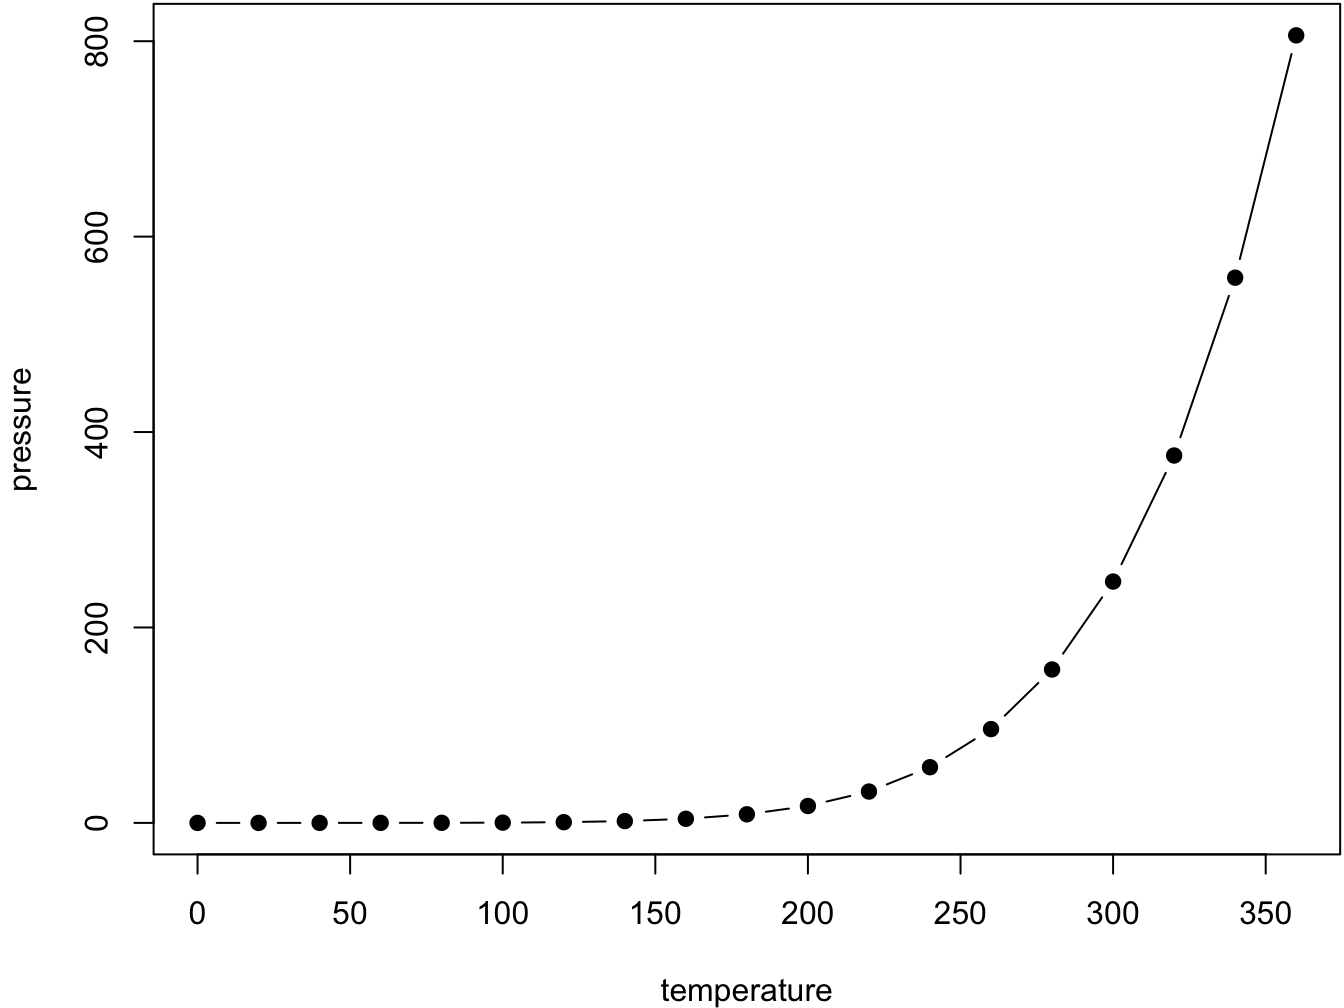
\includegraphics[width=0.8\linewidth]{bookdown-demo_files/figure-latex/nice-fig-1} 

}

\caption{Here is a nice figure!}\label{fig:nice-fig}
\end{figure}

Reference a figure by its code chunk label with the \texttt{fig:}
prefix, e.g., see Figure \ref{fig:nice-fig}. Similarly, you can
reference tables generated from \texttt{knitr::kable()}, e.g., see Table
\ref{tab:nice-tab}.

\begin{Shaded}
\begin{Highlighting}[]
\NormalTok{knitr::}\KeywordTok{kable}\NormalTok{(}
  \KeywordTok{head}\NormalTok{(iris, }\DecValTok{20}\NormalTok{), }\DataTypeTok{caption =} \StringTok{'Here is a nice table!'}\NormalTok{,}
  \DataTypeTok{booktabs =} \OtherTok{TRUE}
\NormalTok{)}
\end{Highlighting}
\end{Shaded}

\begin{table}

\caption{\label{tab:nice-tab}Here is a nice table!}
\centering
\begin{tabular}[t]{rrrrl}
\toprule
Sepal.Length & Sepal.Width & Petal.Length & Petal.Width & Species\\
\midrule
5.1 & 3.5 & 1.4 & 0.2 & setosa\\
4.9 & 3.0 & 1.4 & 0.2 & setosa\\
4.7 & 3.2 & 1.3 & 0.2 & setosa\\
4.6 & 3.1 & 1.5 & 0.2 & setosa\\
5.0 & 3.6 & 1.4 & 0.2 & setosa\\
\addlinespace
5.4 & 3.9 & 1.7 & 0.4 & setosa\\
4.6 & 3.4 & 1.4 & 0.3 & setosa\\
5.0 & 3.4 & 1.5 & 0.2 & setosa\\
4.4 & 2.9 & 1.4 & 0.2 & setosa\\
4.9 & 3.1 & 1.5 & 0.1 & setosa\\
\addlinespace
5.4 & 3.7 & 1.5 & 0.2 & setosa\\
4.8 & 3.4 & 1.6 & 0.2 & setosa\\
4.8 & 3.0 & 1.4 & 0.1 & setosa\\
4.3 & 3.0 & 1.1 & 0.1 & setosa\\
5.8 & 4.0 & 1.2 & 0.2 & setosa\\
\addlinespace
5.7 & 4.4 & 1.5 & 0.4 & setosa\\
5.4 & 3.9 & 1.3 & 0.4 & setosa\\
5.1 & 3.5 & 1.4 & 0.3 & setosa\\
5.7 & 3.8 & 1.7 & 0.3 & setosa\\
5.1 & 3.8 & 1.5 & 0.3 & setosa\\
\bottomrule
\end{tabular}
\end{table}

You can write citations, too. For example, we are using the
\textbf{bookdown} package \citep{R-bookdown} in this sample book, which
was built on top of R Markdown and \textbf{knitr} \citep{xie2015}.

\bibliography{packages.bib,book.bib}


\end{document}
